\chapter{Durchführung}\label{cha:durchfuehrung}
In diesem Kapitel wird die komplette Umsetzung des Besuchs beschrieben. Sämtliche Schritte und Tricks zum Experimentieren, basieren auf dem Experiment Manual von PASCO Scientific \parencite{instructionManualHalogen}. Zuerst werden in \autoref{sec:vorbereitung} die Vorbereitungen erläutert, wie zum Beispiel der richtigen Auswahl der Umgebung oder das Messen des Kondensatorenabstandes. In \autoref{sec:optischesSystem} wird das optische System erklärt und in \autoref{sec:funktionen} die verschiedenen Funktionen der Schalter. Anschliessend wird in \autoref{sec:spannung} und \autoref{sec:Temperatur} beschrieben wie Spannung und Temperatur gemessen werden sollen. Der letzte Abschnitt (\autoref{sec:durchfuehrung}) behandelt das eigentliche Experimentieren, von der richtigen Tröpfchenwahl bis hin zur eigentlichen Berechnung.

\section{Vorbereitung}\label{sec:vorbereitung}
\subsection{Auswahl der Umgebung und Höhe}\label{sub:auswahlUmgebung}
Für die Durchführung des Experiments sind verschiedene Vorbereitungen notwendig. Zunächst gilt es den geeignete Ort auszuwählen. Um das Experiment unter optimalen Bedingungen und mit hoher Präzision durchzuführen, sollte ein möglichst dunklen Raum gewählt werden. Für diese Arbeit stand die Dunkelkammer (Zimmer G10) der Kantonsschule am Burggraben zur Verfügung.

Ein weiterer wichtiger Aspekt betrifft den Untergrund, auf dem das Experiment aufgebaut wird. Im Experimentierkasten befinden sich Verlängerungsstäbe, die das Arbeiten erleichtern sollen. Allerdings sind diese Stäbe nicht besonders stabil, was die Präzision des Experiments negativ beeinflussen könnte. Aus diesem Grund wurde die Plattform auf einen Holzklotz gestellt. Dadurch konnte das Experiment in Augenhöhe und bei aufrechter Körperhaltung durchgeführt werden. Besonders wichtig ist es, sicherzustellen, dass die Plattform eben steht. Das lässt sich mithilfe einer Wasserwaage überprüfen, die auf der Plattform fest verschraubt ist. Sollte die Plattform nicht waagerecht sein, können die verstellbaren Füsse genutzt werden, um sie auszurichten. Durch die Verwendung des Holzklotzes wurde ein stabiler Untergrund geschaffen, der die Grundlage für die Feinjustierung des optischen Systems bot.

\subsection{Kondensatorenabstand messen}\label{sub:kondensatorenabstand}
Im nächsten Schritt der Vorbereitung wird der Abstand zwischen den beiden Kondensatoren gemessen. Dabei ist es von entscheidender Bedeutung, dass die Spannung während des gesamten Vorgangs abgeschaltet bleibt. Zunächst wird das Gehäuse der Betrachtungskammer entfernt. Anschliessend nimmt man vorsichtig die obere Platte ab, gefolgt von der darunterliegenden Kunststoffplatte.

Für die Messung der Dicke der Kunstoffplatte wird die im Experimentierkasten enthaltene Schiebelehre verwendet. Dabei ist es wichtig, die Messung am inneren Rand der Platte durchzuführen, da der äussere Rand eine leicht grössere Dicke aufweist. Der gemessene Wert wird direkt abgelesen und dokumentiert.

\section{Das optische System ausrichten}\label{sec:optischesSystem}
\subsection{Das Betrachtungsfernrohr fokussieren}
Die Betrachtungskammer wird nun wieder zusammengesetzt, wobei das Gehäuse vorerst noch nicht angebracht wird. Der Fokussierdraht auf der Platte ist abzuschrauben und vorsichtig in das Loch in der Mitte der oberen Kondensatorenplatte einzuführen. Anschliessend wird die Halogenlampe angeschlossen. Dazu verbindet man den Stecker des 12~V DC-Transformators mit der Lampe, wodurch diese zu leuchten beginnt.

Der nächste Schritt besteht darin, das Fadenkreuz in den Fokus zu bringen. Hierzu dreht man den Fadenkreuz-Fokussierring, bis das Gitter vollständig und scharf abgebildet wird. Danach wird der Draht durch das Betrachtungsfernrohr betrachtet. Der Tröpfchen-Fokussierring wird so lange zu gedreht, bis der Draht ebenfalls scharf zu sehen ist.

\subsection{Die Halogenlampe einstellen}\label{sub:Halogenlampe}
Mit dem horizontalen Einstellknopf der Halogenlampe wird das Licht auf der horizontalen Ebene korrekt fokussiert. Der optimale Fokus ist erreicht, wenn der rechte Rand des Drahts den höchsten Helligkeitskontrast zur linken Seite aufweist. Anschliessend wird mit dem vertikalen Einstellknopf das Licht so justiert, dass das Zentrum des Gitters bzw. des Fadenkreuzes am hellsten sichtbar ist. Nach Abschluss aller Einstellungen wird der Fokussierdraht vorsichtig wieder in die Vertiefung der Platte eingeschraubt.

\section{Funktionen der Steuerung}\label{sec:funktionen}
\subsection{Kondensatorenspannungsschalter}\label{sub:Spannungsschalter}
Dieser Schalter dient als Spannungswechsler für die beiden Kondensatoren und ermöglicht es, die Richtung des elektrischen Feldes $E$ zu ändern. Der Schalter verfügt über drei verschiedene Positionen: 

\begin{enumerate}
	\item \textbf{plates grounded}: In dieser Position sind beide Kondensatoren ungeladen, so dass keine elektrische Kraft auf die Tröpfchen wirkt.
	\item \textbf{TOP PLATE $-$}: Hier wird die obere Kondensatorenplatte geladen, wodurch das elektrische Feld nach unten gerichtet ist.
	\item \textbf{TOP PLATE $+$}: Die Position wechselt die Richtung des elektrischen Feldes, in dem sie die obere Platte positiv lädt.
\end{enumerate}

\subsection{Der Ionisationsquelle Schalter}\label{sub:ionisationquelle}
Der Schalter für die Ionisationsquelle verfügt auch über drei verschiedene Positionen: 

\begin{enumerate}
	\item \textbf{ionization ON}: Die Abschirmung der Ionisationsquelle ist entfernt, wodurch die Öltröpfchen ionisiert und angestrahlt werden können 
	\item \textbf{spray droplet position}: Diese Position wird verwendet, wenn Öltröpfchen in die Kammer eingesprüht werden. Dabei öfnet sich ein kleines Loch in der Kammer, das der Luft ermöglicht auszuströmen, während das Öl eingesprüht wird.
	\item \textbf{ionization OFF}: In dieser Position wird die Ionisationsquelle vollständig abgeschirmt, sodass keine Alphateilchen in die Kammer gelangen können.
\end{enumerate}

\begin{figure}[ht]
	\begin{center}
		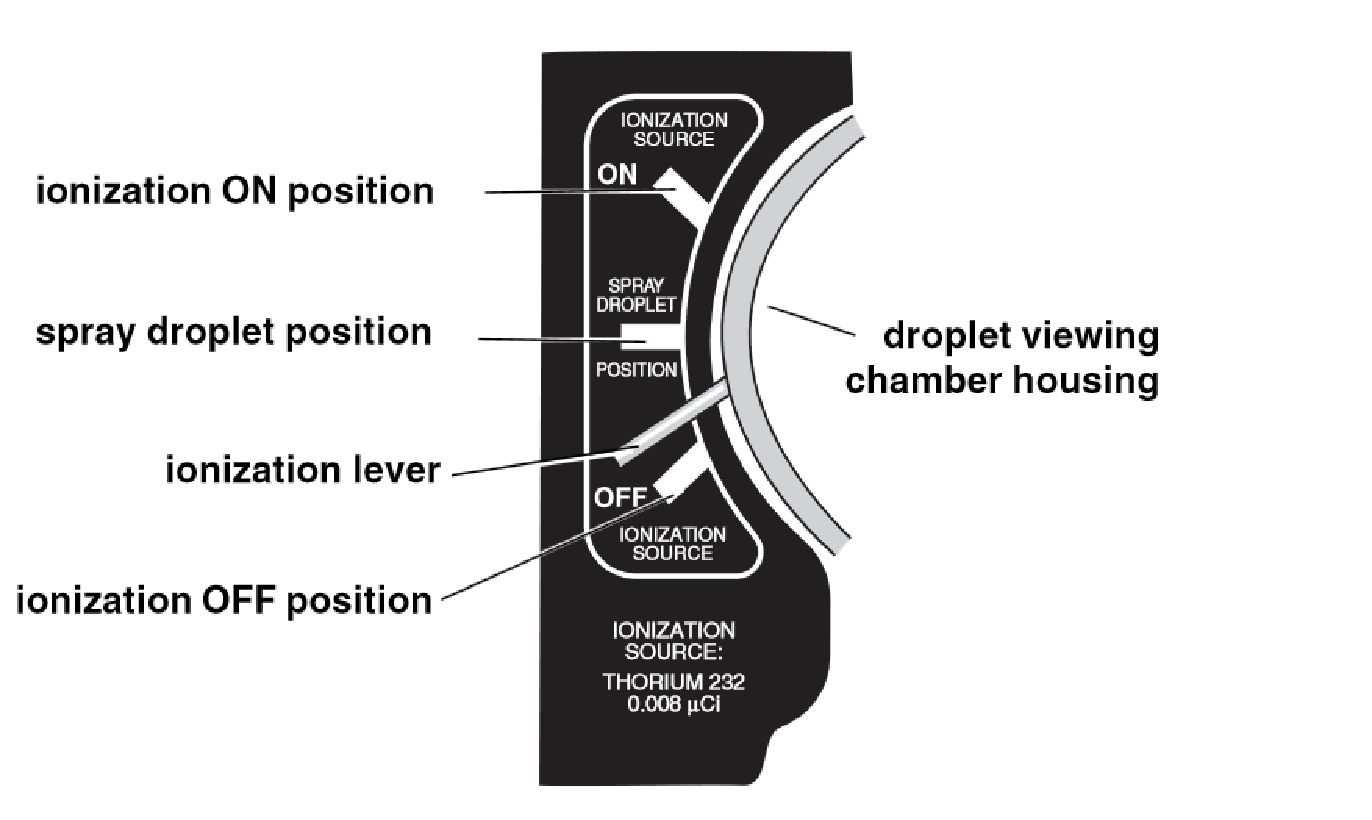
\includegraphics[scale=0.5]{bilder/pdf/Schalterfunktionen.pdf}
		\caption{Schalterpositionen der Ionisationsquelle \parencite[6]{instructionManualHalogen}}
		\label{fig:Schalterpositionen}
	\end{center}
\end{figure}

\section{Messen und Einstellen der Spannung}\label{sec:spannung}
Zunächst wird die Gleichstromquelle über die farbigen Anschlüsse mit der Plattform verbunden. Das digitale Multimeter kann an den Kontakten der Kondensatoren angeschlossen werden. Nach dem Einschalten des Multimeters wird der Modus auf Gleichstromspannung eingestellt. Sobald die Stromquelle eingeschaltet ist, sollte das Multimeter eine Spannung von etwa 500 V anzeigen. Falls dies nicht der Fall ist, muss die Spannung direkt an der Stromquelle entsprechend angepasst werden. Wichtig: Dank den in den Kondensatoren eingebauten grossen Widerstände besteht keine Gefahr eines elektrischen Schocks.

\section{Temperatur in der Tröpfchenkammer}\label{sec:Temperatur}
Die letzte erforderliche Einstellung, vor Beginn des Experiments, besteht darin, die Temperatur innerhalb der Tröpfchenkammer zu messen. Diese ist erforderlich, um die Viskosität der Luft zu bestimmen. Da die Temperatur nicht direkt mit einem Thermometer gemessen werden kann, erfolgt die Bestimmung über den Zusammenhang zwischen dem elektrischen Widerstand der Kondensatoren und der Temperatur. Der Widerstand wird dabei ähnlich wie die Spannung gemessen. Auf der Platte befinden sich speziell Anschlüsse, an die ein digitales Multimeter angeschlossen wird. Das Multimeter sollte auf den Messmodus für elektrischen Widerstand eingestellt werden. Der proportionale Zusammenhang zwischen Temperatur und Widerstand kann einer Tabelle entnommen werden. Es ist unbedingt darauf zu achten, dass die Stromquelle niemals mit den Widerstandsanschlüssen verbunden wird, da dies das Experiment beschädigen könnte. Der Widerstand sollte sich im Bereich von etwa 1 bis 4 Megaohm bewegen.

\begin{figure}[ht]
	\begin{center}
		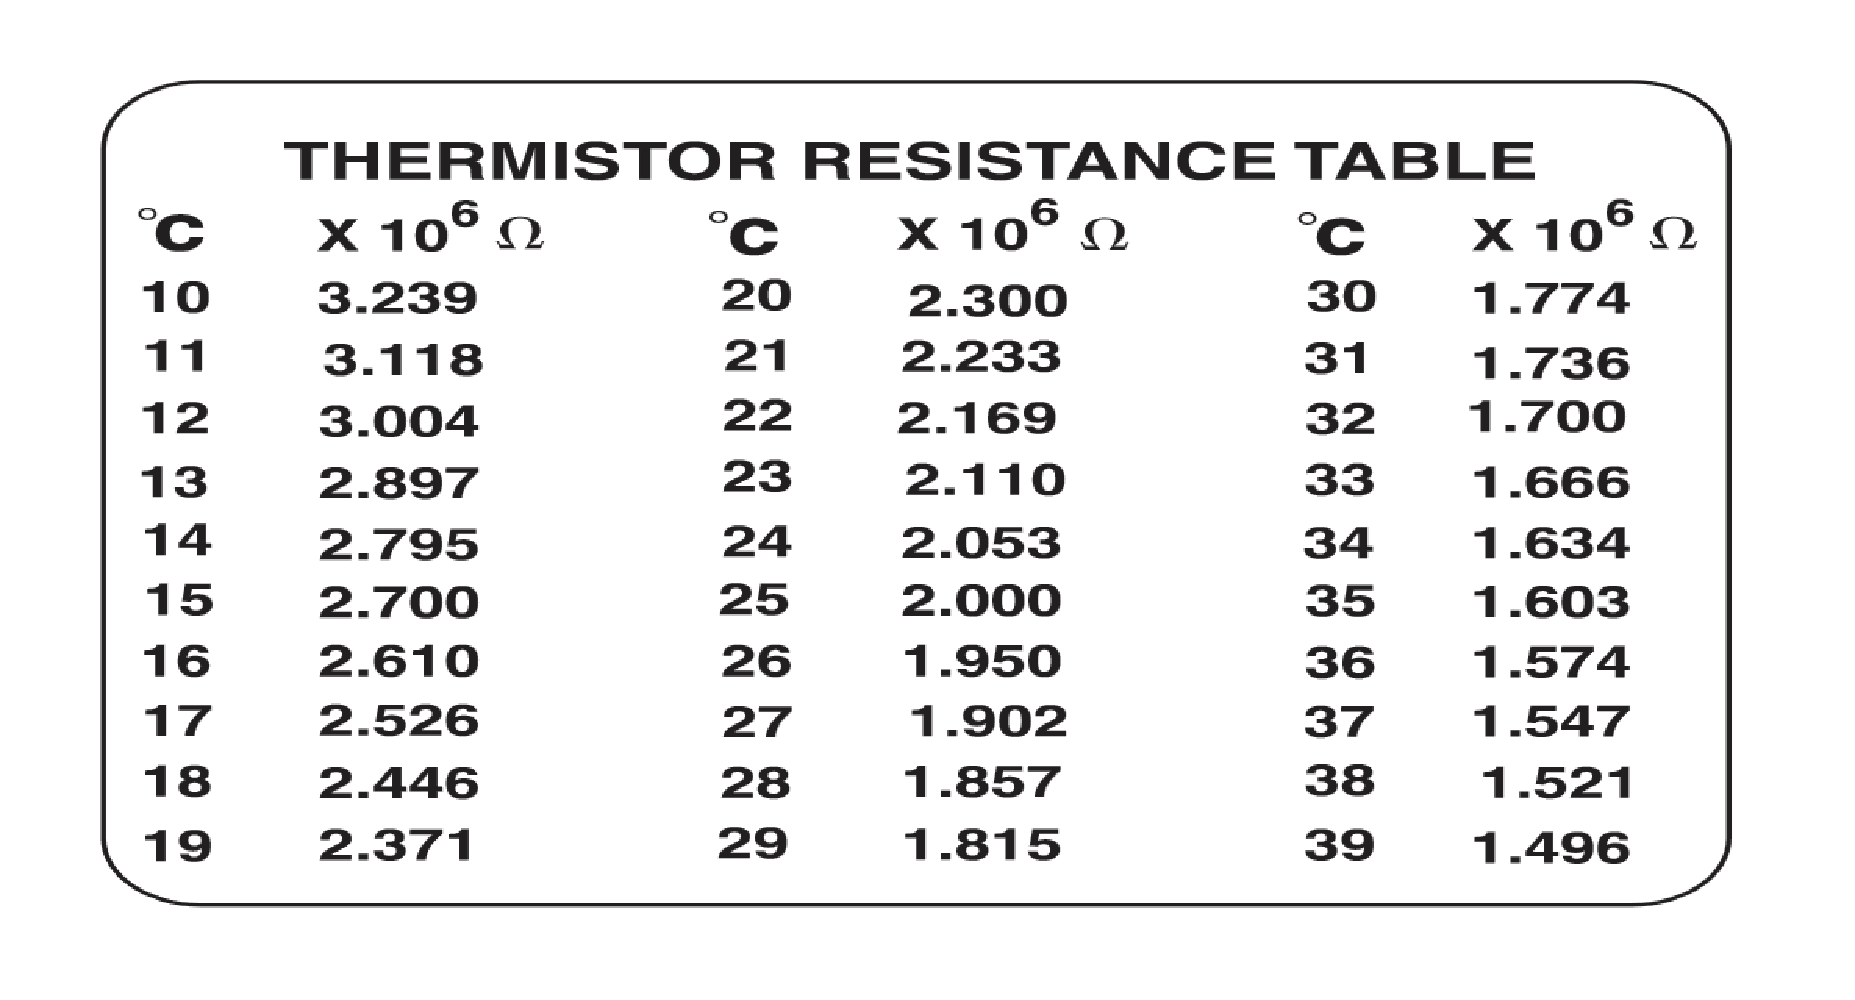
\includegraphics[scale=0.25]{bilder/pdf/TemperaturTabelle.pdf}
		\caption{Abhängigkeit von Temperatur und elektrischer Widerstand \parencite[24]{instructionManual}}
		\label{fig:widerstandTemperatur}
	\end{center}
\end{figure}

\section{Das Experimentieren}\label{sec:durchfuehrung}
Bevor das Experiment starten kann, muss die gesamte Kammer vollständig zusammengesetzt werden. Der Tröpfchenlochschutz wird auf die Öffnung der oberen Platte montiert, um sicherzustellen, dass während des Experiments keine weiteren Tröpfchen in die Betrachtungskammer gelangen. Anschliessend werden die Spannung und die Temperatur noch einmal überprüft, um sicherzustellen, dass alle Bedingungen für den Versuch erfüllt sind. Erst danach kann mit dem Experiment fortgefahren werden.

\subsection{Tröpfchen einsprühen}\label{sub:tröpfchensprühen}
Der erste Schritt besteht in der Vorbereitung des Ölsprühers. Dazu wird Mineralöl, mit bekannter Dichte (z.B. das zugehörige Squibb \#5597 Mineral Oil mit Dichte: $886 kg/m^3$), in den Zerstäuber gefüllt. Anschliessend wird geprüft, ob der Zerstäuber ordnungsgemäss Tröpfchen erzeugt. Dazu wird mehrmals schnell und mit leichtem Druck auf das Kissen des Zerstäubers gedrückt, bis auf einem Papier kleine Tröpfchen sichtbar werden.
\begin{figure}[h]
		\centering
		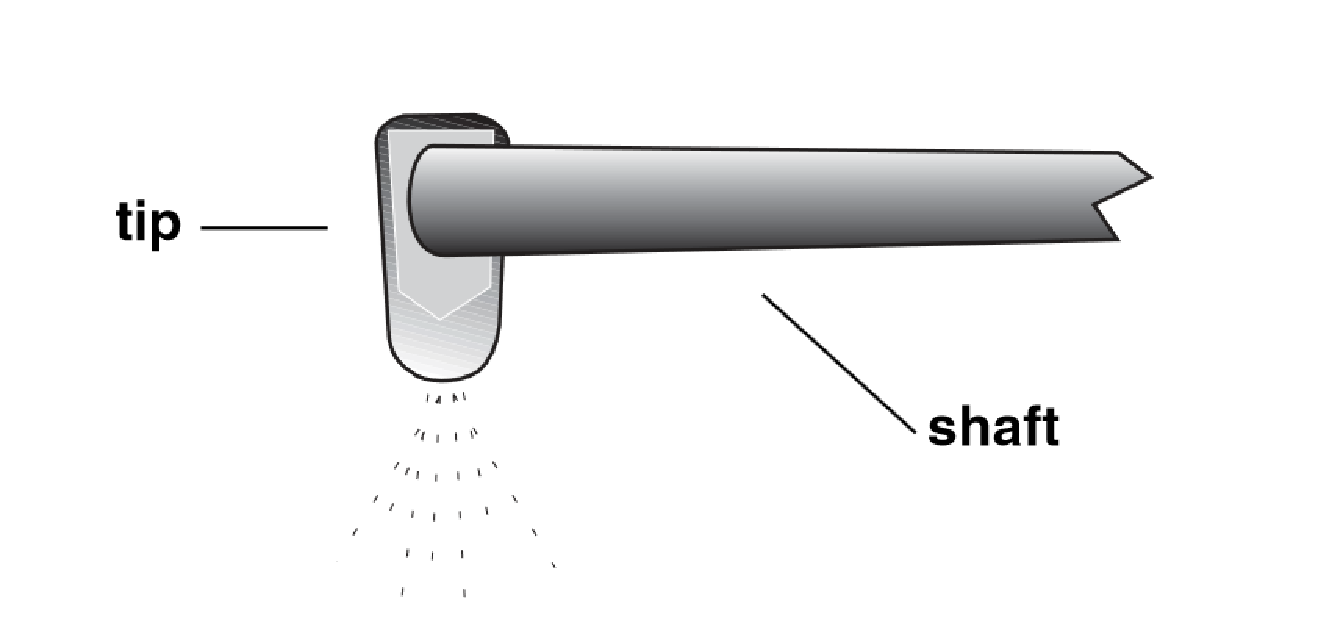
\includegraphics[scale=0.25]{bilder/pdf/zerstauberSpitze.pdf}
		\caption{Korrekte Position von der Spitze zur Achse \parencite[7]{instructionManualHalogen}}
		\label{fig:zerstauberSpitze}
\end{figure}

\noindent Die Spitze des Zerstäubers muss nach unten schauen. Genau 90° zur Achse. (siehe \autoref{fig:zerstauberSpitze})

Nach diesem Schritt muss der Schalter der Ionisationsquelle auf die \textbf{spray droplet} Position gestellt werden, um sicherzustellen, dass während des Einsprühens die Luft aus der Kammer entweichen kann. Da die Spitze des Zerstäubers nach unten zeigt, kann dieser nun direkt in das vorgesehene Loch auf dem Deckel des Gehäuses eingeführt werden. Nun sollte durch das Betrachtungsfernrohr geschaut werden, während gleichzeitig kräftig auf das Kissen des Zerstäubers gedrückt wird. Anschliessend werden mit schwächeren, kleineren Stössen die Tröpfchen ins Sichtfeld des Betrachters gebracht. Sobald eine Ansammlung von kleinen goldenen Punkten sichtbar wird, muss der Schalter auf die \textbf{OFF} Position zurückgesetzt werden.

Das Einsprühen der Tröpfchen kann zu Beginn eine Herausforderung darstellen und wird vermutlich nicht beim ersten Versuch erfolgreich sein. Es gibt keine festgelegte Technik für den Umgang mit dem Zerstäuber; der Experimentator muss eine eigene Methode entwickeln, um den Zerstäuber effizient zu bedienen. Dieser Vorgang kann viel Zeit in Anspruch nehmen. In dieser Arbeit stellte sich heraus, dass es am besten funktionierte, den Zerstäuber einmal kräftig zu drücken und danach kleinere, schwächere Stösse zu verabreichen.

Falls zu viele Tröpfchen im Sichtfeld sichtbar sind, empfiehlt es sich, drei bis vier Minuten zu warten, bis die meisten Tröpfchen verschwunden sind. Danach kann das Experiment in Ruhe fortgesetzt werden.

\subsection{Auswahl des richtigen Tröpfchens}\label{sub:auswahlTropfen}
Von den sichtbaren Tröpfchen sollte eines ausgewählt werden, dessen Fallgeschwindigkeit etwa zwischen $0.02$ und $0.05$ mm/s liegt, wenn der Schalter der Kondensatoren auf \textbf{plates grounded} gestellt ist. Die Fallgeschwindigkeit sollte so gewählt werden, dass sich das Tröpfchen mit dem Schalter vertikal bewegen lässt. Diese spezifische Beschreibung der Fallgeschwindigkeit ist schwierig genau zu messen. Ein hilfreicher Hinweis: Ein Tröpfchen, das etwa 15 Sekunden benötigt, um die Distanz von $0.5$ mm zwischen zwei Hauptlinien des Gitters zu durchqueren, bewegt sich mit einer Geschwindigkeit von ungefähr $0.03$ mm/s.

Sollten immer noch zu viele Tröpfchen im Sichtfeld sichtbar sein, kann es hilfreich sein, die Kondensatoren für kurze Zeit zu laden, um die meisten Tröpfchen zu entfernen. Da nicht alle Tröpfchen eine Nettoladung aufweisen und daher nicht beeinflusst werden, kann der Ionisationsschalter für drei bis fünf Sekunden in die \textbf{ON} Position geschaltet werden, um sicherzustellen, dass sich alle Tröpfchen bewegen lassen.

Sobald ein geeignetes Tröpfchen gefunden wurde, dessen Fallgeschwindigkeit innerhalb der gewünschten Grössenordnung liegt, kann der Fokussierring verwendet werden, um das Tröpfchen weiter zu schärfen. Dies entlastet die Augen des Experimentators und ermöglicht eine längere Beobachtungsdauer. Der beste Fokus ist erreicht, wenn das Tröpfchen wie eine goldene Nadelspitze erscheint.

\subsection{Daten sammeln mit der Fall und Steigzeit}\label{sub:datenFallundSteig}
Zur Bestimmung der Ladung eines Öltröpfchens müssen sowohl die Steiggeschwindigkeit (bei geladenen Kondensatoren) als auch die Sinkgeschwindigkeit (bei nicht geladenen Kondensatoren) gemessen werden. Die genaueste Messung erfolgt, indem die Zeit gemessen wird, die das Tröpfchen benötigt, um von der ersten grossen Linie bis zur zweiten grossen Linie zu gelangen. Diese Linien sind exakt $0.5$ mm voneinander entfernt. Die Geschwindigkeit $v$ kann dann mit der Formel $v = \frac{s}{t}$ berechnet werden, wobei $s$ die zurückgelegte Strecke und $t$ die benötigte Zeit ist. Ein Beispiel: Wenn ein Tröpfchen $15$ Sekunden benötigt, um die Strecke von $0.5$ mm zu überwinden, ergibt sich die Geschwindigkeit zu $v = \frac{0.5,\text{mm}}{15,\text{s}} = 0.033,\text{mm/s} = 3.3 \cdot 10^{-5},\text{m/s}$.

Für präzisere Ergebnisse sollte die Geschwindigkeit eines Tröpfchens etwa 5 bis 15 Mal gemessen werden.

Nach der ersten Messung kann die Ladung des Tröpfchens provisorisch geschätzt werden. Falls die gemessene Ladung mehr als das Fünffache der Elementarladung beträgt, sollte für die weiteren Messungen ein langsameres Tröpfchen gewählt werden.

Anschliessend sollten neue Tröpfchen eingesprüht und die Geschwindigkeiten erneut gemessen werden, bis das Tröpfchen seine Ladung spontan ändert oder aus dem Sichtfeld verschwindet. Die Ladung eines Tröpfchens kann durch den Ionisationsschalter verändert werden. In diesem Schritt sollten die Messungen so oft wie möglich wiederholt werden, um eine möglichst präzise Bestimmung der Ladung zu erhalten. Sollte die Beobachtung durch Ermüdung beeinträchtigt werden, können alternative Messgrössen wie die Spannung, die Zähigkeit der Luft, die Dichte des Öls und der Luftdruck aufgezeichnet werden. Alle Messdaten sollten in einer Tabelle dokumentiert werden, bevor mit der Berechnung der Ladungen aus den einzelnen Messungen fortgefahren wird.

\subsection{Methode für die Berechnung der Ladung}\label{sub:methodeBerechnung}
Mit der Formel in \autoref{eq:qRadius} kann zuerst der Radius $a$ berechnet werden:
\begin{equation*}
	a \ = \ \sqrt{\left( \frac{b}{2p}\right)^2 + \frac{9\eta v_f}{2\rho g}} - \frac{b}{2p}
\end{equation*}

\noindent Anschliessend kann die Masse $m$ des Tröpfchens berechnet werden, indem man die Formel für den Radius in den Ausdruck für die Masse einsetzt:
\begin{equation*}
	\begin{split}
		m & \ = \ \frac{4}{3}\pi a^3 \rho \\
		& \ = \ \frac{4}{3}\pi \left( \sqrt{\left( \frac{b}{2p}\right)^2 + \frac{9\eta v_f}{2\rho g}} - \frac{b}{2p} \right)^3 \rho
	\end{split}
\end{equation*}

\noindent Der letzte Schritt besteht darin, die Masse $m$ in der \autoref{eq:hauptgleichung} zu substituieren:
\begin{equation*}
	\begin{split}
		q & \ = \ \frac{m g (v_f + v_r)}{Ev_f} \\
		& \ = \ \frac{4}{3} \pi \rho g \left( \sqrt{\left( \frac{b}{2p}\right)^2 + \frac{9\eta v_f}{2\rho g}} - \frac{b}{2p} \right)^3 \frac{(v_f + v_r)}{Ev_f}
	\end{split}
\end{equation*}

\noindent Wenn man nun $E$ mit der \autoref{eq:elektrischeFeldstärke} ersetzt, erhält man die Ladung $q$ eines Tröpfchens:
\begin{equation*}
	q_{tröpfchen} \ = \ \frac{4}{3} \pi \rho g \left( \sqrt{\left( \frac{b}{2p}\right)^2 + \frac{9\eta v_f}{2\rho g}} - \frac{b}{2p} \right)^3 \frac{d(v_f + v_r)}{Vv_f}
\end{equation*}







